\section{Porówannie wykorzystanych algorytmów}

\subsection{Parametry sprzętowe}

Badania zostały przeprowadzone na kilku węzłach spośród dostępnego na
Politechnice klastra obliczeniowego. Jednakże każdy pojedynczy pomiar
odbywał się przy obliczeniach wykonywanych na jednaj maszynie.
Każda z jednostek klastra posiada następujące parametry sprzętowe:
\begin{itemize}
 \item CPU : Intel(R) Xeon(R) CPU X3230@2.66GHz
 \item Pamięć : 4GB
\end{itemize}
Pomimo, że procesory dysponowały czterema rdzeniami, nie zdecydowano się
na zrównoleglenie procesu obliczeń oraz zrównolelenie samego procesu
wykonywania testów. W zamian za to, każdy typ algorytmu testowany był
na innej maszynie fizycznej.

\subsection{Dane wejściowe}

Wygenerowane na potrzeby testów dane charakterysowały się
losowym rozmieszczeniem punktów. Generator instancji ze względu na
asymetrię problemu musiał uwzględniać różne odległości między punktami
w zależności od kierunku łuku w grafie. Tak więc początkowo losowane były
pozycje punktów. Na podstawie pozycji wyznaczana była odległość
zgodnie z kierunkiem wierzchołków od $u$ do $v$. Odległość od $v$ do $u$
z kolei była wyznaczana na podstawie poprzednio wyliczonej wartości
jednakże była modyfikowana o pewną losową wartość $\pm rand()$.


Dane wejściowe posiadały w zależności od konfiguracji od 50 do 400
wierzchołków. Przygotowane dane były wczytywane przez program z wcześniej
utworzonych plików, a na podstawie położenia zaczytanych wierzchołków
oraz odległości między nimi wykonywane były  obliczenia.

Pomimo utworzenia generatora instancji problemu oraz funkcji wyznaczania
ograniczenia dolnego, zdecydowano się wykorzystać istniejące
instancje problemu pobrane ze strony internetowej
\url{http://comopt.ifi.uni-heidelberg.de/software/TSPLIB95/}. Przedstawione
instancje problemu były już wielokrotnie analizowane przez osoby
tworzące różnorakie rozwiązania problemu ATSP. Na stronie udostępnione
są wyniki optymalne dla poszczególnych instancji, co ułatwia porównywanie
algorytmów.

Wszystkie testowane algorytmy uruchamiane
były po 10 razy dla każdej z testowanych instancji. Kolejne uruchomienia
różniły się rozwiązaniem początkowym, dlatego można się było spodziewać
różnych wyników dla każdego spośród wywołań. Algorytm 
losowy był uruchamiony dodatkowo dla każdej instancji po 10 razy ze zmiennym
limitem losowań w granicach 20~000 do 200~000 powtórzeń.

\begin{center}

\begin{tabular}{lcccccccccc}

\toprule
\multirow{2}{*}{Instancja} & {Rozw.} &
\multicolumn{2}{c}{Random} & \multicolumn{2}{c}{Greedy} &
\multicolumn{2}{c}{Steepest} & Własne\\
 &  Optymalne & Wynik & Czas$[s]$& Wynik & Czas$[s]$ & Wynik & Czas$[s]$& Wynik \\
\toprule
%% All data must appear between the \startdata and \enddata commands
br17 & 39 & 60 & 0.02 & 45.1 & 0 & 46.9 & 0 & 86.3 \\
\midrule
ft53 & 6905 & 21078.3 & 0.08 & 10411.6 & 0.14 & 11004.5 & 0.34 & 9324.9 \\
\midrule
ft70 & 38673 & 65184 & 0.1 & 45568.7 & 0.32 & 46089.7 & 1.02 & 42998.8 \\
\midrule
ftv170 & 2755 & 23188.6 & 0.24 & 6894.5 & 10.18 & 7437.2 & 42.28 & 3937.6 \\
\midrule
ftv33 & 1286 & 3329.5 & 0.05 & 1826.6 & 0.02 & 1765.5 & 0.05 & 1737.6 \\
\midrule
ftv35 & 1473 & 3764.9 & 0.05 & 2163.7 & 0.02 & 2061.1 & 0.07 & 1892.7 \\
\midrule
ftv38 & 1530 & 3997.5 & 0.05 & 2184.1 & 0.04 & 2164.9 & 0.1 & 1931.3 \\
\midrule
ftv44 & 1613 & 4821 & 0.06 & 2439.3 & 0.06 & 2466.5 & 0.17 & 2172.2 \\
\midrule
ftv47 & 1776 & 5410.4 & 0.07 & 2735.9 & 0.07 & 2632.4 & 0.21 & 2467.2 \\
\midrule
ftv55 & 1608 & 5895.4 & 0.08 & 2684.5 & 0.13 & 2691.1 & 0.4 & 2282.5 \\
\midrule
ftv64 & 1839 & 7259.2 & 0.09 & 3124.7 & 0.23 & 3231.9 & 0.73 & 2505 \\
\midrule
ftv70 & 1960 & 8086.8 & 0.11 & 3438.3 & 0.35 & 3427.8 & 1.13 & 2502.2 \\
\midrule
kro124p & 36230 & 158131.5 & 0.14 & 57832.9 & 1.91 & 63434.7 & 5.83 & 46915.7 \\
\midrule
rbg323 & 1326 & 5695.8 & 0.46 & 1678.4 & 109.32 & 1718.5 & 470.02 & 1747.1 \\
\midrule
rbg358 & 1163 & 6369.2 & 0.51 & 1582.7 & 154.66 & 1606.9 & 737.28 & 1789.1 \\
\midrule
rbg403 & 2465 & 7144.2 & 0.57 & 2761.8 & 244.57 & 2764.9 & 1016.9 & 3524.3 \\
\midrule
rbg443 & 2720 & 7680.3 & 0.63 & 3020.3 & 371.88 & 3063.5 & 1513.56 & 3899.2 \\
\midrule
ry48p & 14422 & 40759.2 & 0.07 & 18890.7 & 0.12 & 19868.8 & 0.27 & 17561.7 \\
\bottomrule
\end{tabular}
\end{center}

\begin{figure}
\begin{center}
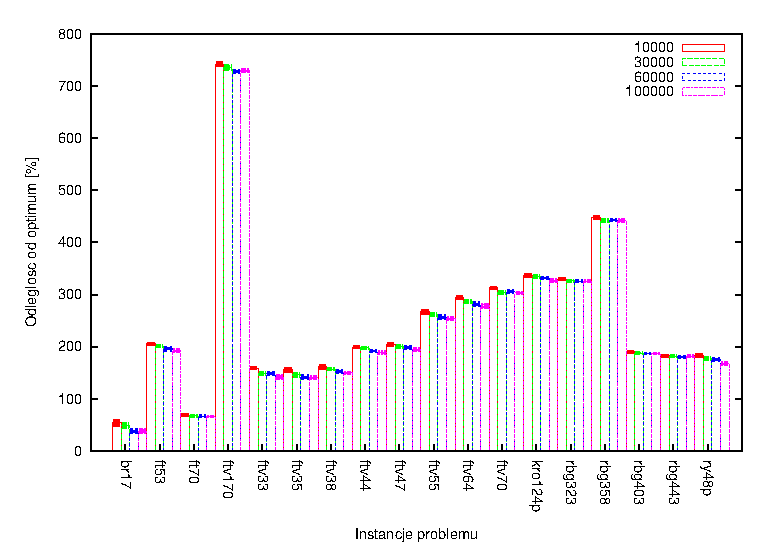
\includegraphics[width=0.9\textwidth]{wykresy/random1}
\end{center}
\caption{Wyniki odległości od optimum dla algorytmu losowego.}
\label{random1}
\end{figure}

\begin{figure}
\begin{center}
\includegraphics[width=0.9\textwidth]{wykresy/greedy_1}
\end{center}
\caption{Wyniki odległości od optimum dla algorytmu $Greedy$.}
\label{greedy_1}
\end{figure}

\begin{figure}
\begin{center}
\includegraphics[width=0.9\textwidth]{wykresy/steepest1}
\end{center}
\caption{Wyniki odległości od optimum dla algorytmu $Steepest$.}
\label{steepest1}
\end{figure}

\begin{figure}
\begin{center}
\includegraphics[width=0.9\textwidth]{wykresy/greedy2_1}
\end{center}
\caption{Wyniki odległości od optimum dla algorytmu autorskiego.}
\label{greedy2_1}
\end{figure}

\begin{figure}
\begin{center}
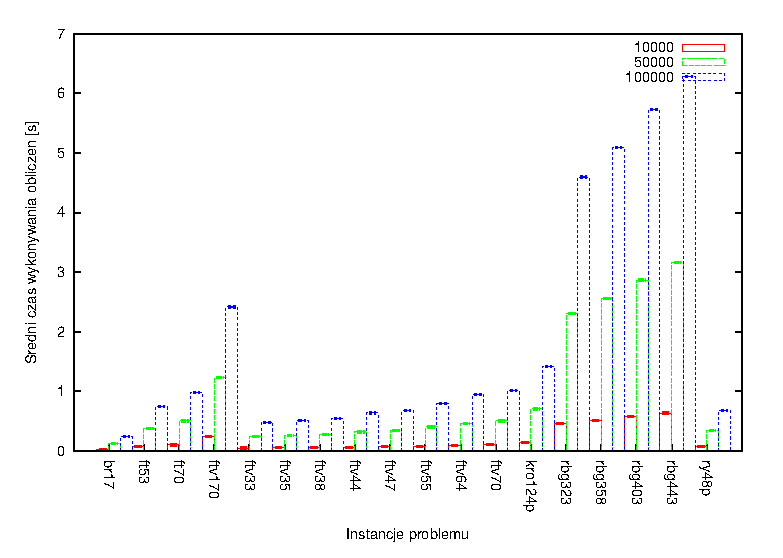
\includegraphics[width=0.9\textwidth]{wykresy/random2}
\end{center}
\caption{Wyniki czasu obliczeń dla algorytmu losowego, w zależności
od liczby losowań.}
\label{random2}
\end{figure}


\begin{figure}
\begin{center}
\includegraphics[width=0.9\textwidth]{wykresy/steepest_greedy_better_solutions}
\end{center}
\caption{Liczba popraw wartości rozwiązania podczas przebiegu algorytmu.}
\label{steepest_greedy_better_solutions}
\end{figure}

\begin{figure}
\begin{center}
\includegraphics[width=0.9\textwidth]{wykresy/steepest_greedy_czas}
\end{center}
\caption{Czas przetwarzania dla algorytmów $Greedy$ oraz $Steepest$.}
\label{steepest_greedy_czas}
\end{figure}


\begin{figure}
\begin{center}
\includegraphics[width=0.9\textwidth]{wykresy/steepest_greedy_czas_log}
\end{center}
\caption{Czas przetwarzania dla algorytmów $Greedy$ oraz $Steepest$ naniesiony
na skali logarytmicznej}
\label{steepest_greedy_czas_log}
\end{figure}

\begin{figure}
\begin{center}
\includegraphics[width=0.9\textwidth]{wykresy/steepest_greedy_steps}
\end{center}
\caption{Ilość kroków wykonanych przez algorytm $Greedy$ oraz $Steepest$.}
\label{steepest_greedy_steps}
\end{figure}

\begin{figure}
\begin{center}
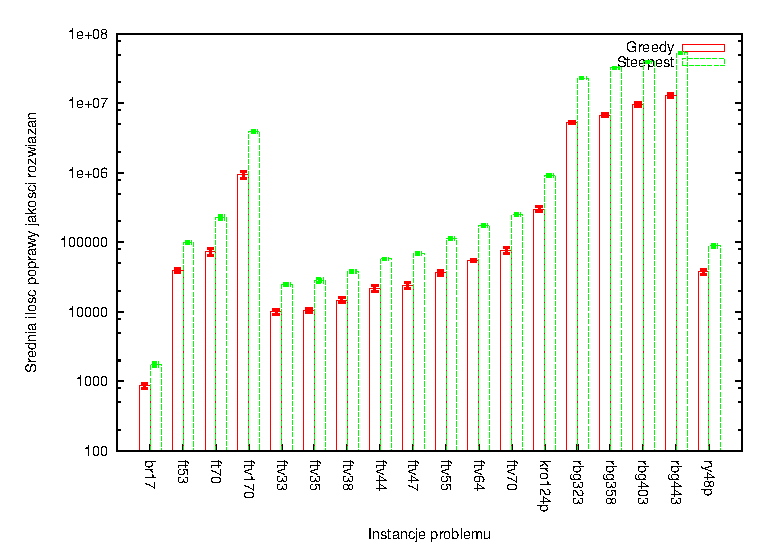
\includegraphics[width=0.9\textwidth]{wykresy/steepest_greedy_visits}
\end{center}
\caption{Ilość odwiedzonych przez algorytmy $Greedy$ oraz $Steepest$
rozwiązań.}
\label{steepest_greedy_visits}
\end{figure}

\begin{figure}
\begin{center}
\includegraphics[width=0.9\textwidth]{wykresy/steepest_greedy_jc}
\end{center}
\caption{Miara $jakosc/czas$ dla algorytmów $Greedy$ oraz $Steepest$.}
\label{steepest_greedy_jc}
\end{figure}

\subsection{Jakość rozwiązań}

Po wykonaniu eksperymentów obliczeniowych można dokonać analizy jakości
rozwiązań otrzymanych przez poszczególne algorytmy. Dzięki posiadanym
wartościom miary długości scieżek optymalnych dostępnych na
stronie internetowej $TSPLIB$ możliwe jest określenie dokładności
rozwiązań przybliżonych zwracanych przez algorymty heurystyczne. Patrząc
na otrzymane wyniki można z łatwością stwierdzić, że zaprezentowane
heurystyki zwracają dość dobre wyniki. Wyjątkiem jest algorytm
losowy, dla którego jakość rozwiązań bardzo odbiega od oczekiwanych
rezultatów.

\subsection{Odległość od optimum}

Miarą dokładności rozwiązań jest odległość od optimum
która wyliczana jest jako proporcja wielkości otrzymanej
do wartości optymalnej. Dokładniej rzecz biorąc, jakość rozwiązania
może zostać zapisana w postaci wzoru zamieszczonego poniżej.


$$
\eta =
\left (\frac{f_{obliczone}}{f_{optymalne}} - 1\right )\cdot 100 \%
$$

Na wykresach zamieszczonych poniżej przedstawione są wyniki dokładności
uzyskanych rezultatów dla poszczególnych algorytmów. Oczywiste wydaje się,
że im mniejsza wartość odległości od optimum, tym jakość rozwiążania
jest większa.



\subsection{Czas działania}

W czasie wykonywania eksperymentu obliczeniowego okazało się, że
rozwiązanie autorskie pozwala na znalezienie rozwiązania w bardzo
krótkim czasie, dlatego w niniejszym raporcie czas wykonania
został pominięty. Jest on niewspółmiernie niski w porównaniu do
czasu wykonania pozostałych algorytmów.

Ze względu na bardzo duże zróżnicowanie czasu wykonywania algorytmów
w zależności od rozmiaru instancji, oprócz wyników przedstawionych
na standardowej osi liczbowej, wykonano także wykresy na skali
logarytmicznej, co można zauważyć na rysunku \ref{steepest_greedy_czas}.

\subsection{Jakość/czas}

Ze względu na fakt, bardzo krótkiego czasu wykonania algorytmu
autorskiego, o którym wspomniano w poprzedniej części w czasie analizy
parametru \emph{jakość/czas} nie uwzględniano tego algorytmu.

Do analizy pozostałych przypadków wykorzystano wartości zdefiniowane
w postaci poniższego wzoru, charakteryzującego stosunek \emph{jakość/czas}.

$$
	\lambda = t \cdot \eta
$$

gdzie $\eta$ - jakość rozwiązania; $t$ - czas działania algorytmu.

Nietrudno zauważyć, że rozumienie powyższego parametru jest niezgodne
z intuicyjnym podejściem. Paramter jakość/czas wydawałoby się powinien
przyjmować wysokie wartości w przypadku dobrej jakości rozwiązań. W
przedstawionym przypadku jest jednak inaczej, a więc im mniejsza
wartość tym lepsze okazuje się rozwiązanie. Wyniki
dla rezultatów otrzymanych w przypadku algorytmu $Steepest$ oraz
$Greedy$ zostały zaprezentowane na rysunku nr \ref{steepest_greedy_jc}.

\subsection{Średnia ilość kroków algorytmów}

Kolejną wartością, na którą zwrócono uwagę w czasie eksperymentu
obliczeniowego jest ilość kroków, które zostały wykonane zgodnie
z działaniem algorytmu. Dla algorytmu autorskiego oraz losowego
nie istnieje potrzeba wprowadzania takiej wartości, gdyż ilość
kroków we wspomnianych algorytmach jest znana na początku działania
algorytmu. W przypadku rozwiązania autorskiego ilość krotków jest
równa ilości węzłów w strukturze, natomiast w przypadku algorytmu
losowego jest ustalana przez użytkownika w momencie uruchomienia.
